\documentclass{beamer}
\usepackage{color}
\newcommand{\onto}[1]{{\texttt{\color{blue}#1}}}
\newcommand{\mycomment}[1]{}


% There are many different themes available for Beamer. A comprehensive
% list with examples is given here:
% http://deic.uab.es/~iblanes/beamer_gallery/index_by_theme.html
% You can uncomment the themes below if you would like to use a different
% one:
%\usetheme{AnnArbor}
%\usetheme{Antibes}
%\usetheme{Bergen}
%\usetheme{Berkeley}
%\usetheme{Berlin}
%\usetheme{Boadilla}
%\usetheme{boxes}
%\usetheme{CambridgeUS}
%\usetheme{Copenhagen}
%\usetheme{Darmstadt}
%\usetheme{default}
%\usetheme{Frankfurt}
%\usetheme{Goettingen}
%\usetheme{Hannover}
%\usetheme{Ilmenau}
%\usetheme{JuanLesPins}
%\usetheme{Luebeck}
\usetheme{Madrid}
%\usetheme{Malmoe}
%\usetheme{Marburg}
%\usetheme{Montpellier}
%\usetheme{PaloAlto}
%\usetheme{Pittsburgh}
%\usetheme{Rochester}
%\usetheme{Singapore}
%\usetheme{Szeged}
%\usetheme{Warsaw}

\title{API4KP Metamodel}

% A subtitle is optional and this may be deleted
\subtitle{A Meta-API for Heterogeneous Knowledge Platforms}

\author{T.~Athan\inst{1} 
\and R.~Bell\inst{2}
\and E.~Kendall\inst{3}
\and A.~Paschke\inst{4}
\and D.~Sottara\inst{5}
}
% - Give the names in the same order as the appear in the paper.
% - Use the \inst{?} command only if the authors have different
%   affiliation.

\institute[Athan Serv/Raytheon/Thematix/FUB/ASU] % (optional, but mostly needed)
{
 \inst{1}%
 Athan Services (athant.com), West Lafayette, Indiana, USA
\and
 \inst{2}%
 Raytheon, Fort Wayne, Indiana, USA
\and
 \inst{3}%
 Thematix Partners LLC, New York, New York, USA
\and
 \inst{4}%
 AG Corporate Semantic Web, Freie Universitaet Berlin, Germany
\and
 \inst{5}%
 Department of Biomedical Informatics, Arizona State University, USA
}
% - Use the \inst command only if there are several affiliations.
% - Keep it simple, no one is interested in your street address.

\date{RuleML Symposium, Berlin, August 2015}
% - Either use conference name or its abbreviation.
% - Not really informative to the audience, more for people (including
%   yourself) who are reading the slides online

\subject{Standards for Knowledge Platforms}
% This is only inserted into the PDF information catalog. Can be left
% out. 

% If you have a file called "university-logo-filename.xxx", where xxx
% is a graphic format that can be processed by latex or pdflatex,
% resp., then you can add a logo as follows:

% \pgfdeclareimage[height=0.5cm]{university-logo}{university-logo-filename}
% \logo{\pgfuseimage{university-logo}}

% Delete this, if you do not want the table of contents to pop up at
% the beginning of each subsection:
\AtBeginSubsection[]
{
  \begin{frame}<beamer>{Outline}
    \tableofcontents[currentsection,currentsubsection]
  \end{frame}
}

% Let's get started
\begin{document}

\begin{frame}
  \titlepage
\end{frame}

\begin{frame}{Outline}
  \tableofcontents
  % You might wish to add the option [pausesections]
\end{frame}

% Section and subsections will appear in the presentation overview
% and table of contents.
\section{Scope}
\begin{frame}{A Meta-API for Knowledge Platforms}

\begin{columns}[c]
\column{2.2in}
\begin{itemize}
\item A Meta-API is a platform-independent model (PIM) for a family of APIs in specific languages, also called PSMs (platform-specific models).
\end{itemize}
\column{1.5in}
\begin{itemize}
\item API4KP provides a PIM for the external APIs of Knowledge Platforms.
\end{itemize}
\end{columns}
\begin{figure}[ht!]
\centering
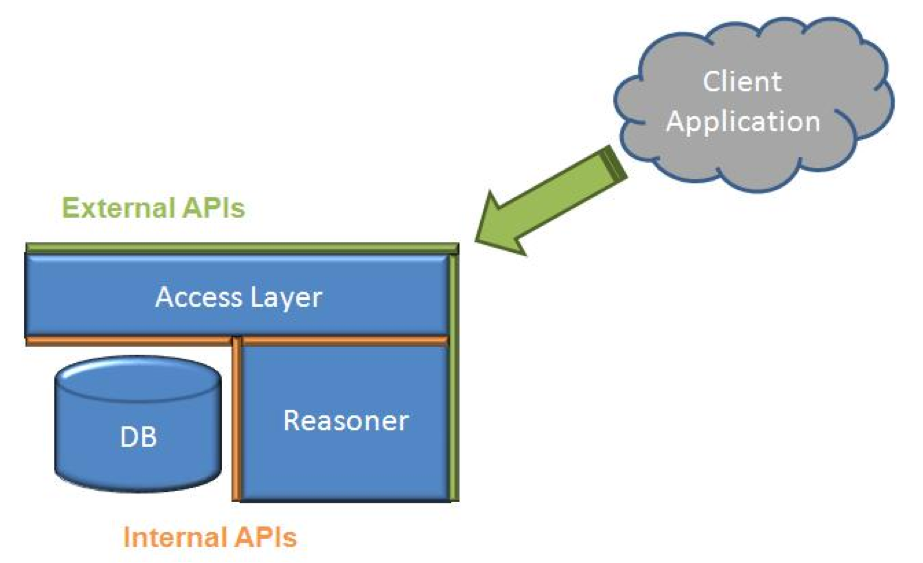
\includegraphics[width=60mm]{diagrams/SimpleKnowledgePlatformArchitecture.png}
\caption{A Monolithic Knowledge Platform architecture.}
\end{figure}  

\end{frame}


\section{Usecase: The Connected Patient System}

\begin{frame}{The Connected Patient System I: Streaming Data and Query Results}
  \begin{itemize}
  \item {Input is obtained from biomedical devices through publish-subscribe.
  }
  \item {Streaming data arrives in various formats, including
     \begin{itemize}
     \item device-specific formats, e.g. XMPP
     \item RDF graphs
     \end{itemize}
  }
  \item Data vocabularies are defined in RDFS, OWL or CL ontologies.
  \item Healthcare providers submit SPARQL queries, receiving streamed incremental results, updated as new data arrives.
  \end{itemize}
  \begin{figure}[ht!]
\centering
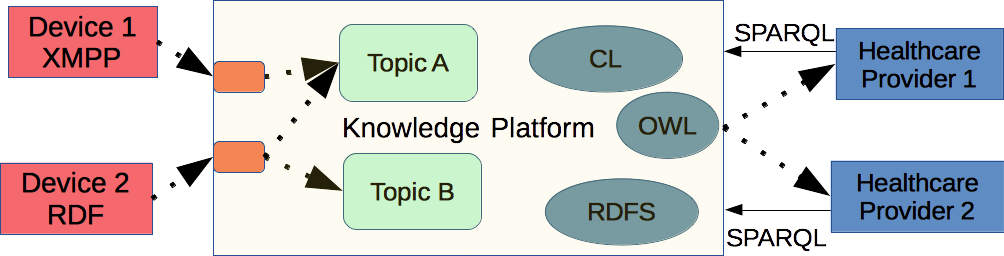
\includegraphics[width=100mm]{diagrams/ConnectedPatient1.png}
\caption{A Heterogeneous Knowledge Platform architecture.}
\end{figure}  
\end{frame}
  
  
\begin{frame}{The Connected Patient System II: CDS}
  \begin{itemize}
  \item A Clinical Decision Support System (CDS) is defined using event-condition-action (ECA) rules, reacting to
     \begin{itemize}
     \item simple events (e.g. a vital parameter exceeding a threshold)
     \item complex events (e.g. a decreasing trend in the average daily physical activity)
     \end{itemize}
     intervening with alerts and reminders.
  \item A failure of response to an alert leads to escalation to another recipient.
  \end{itemize}
\end{frame}
  
  
\begin{frame}{The Connected Patient System III: Case History}
  \begin{itemize}
  \item The system maintains a stateful representation for patients qualifying for clinical pathways.
  \item Clinicians check for compliance with planned orders.
  \item As medical guidelines evolve, the logic of the pathway may need revision: queries to the patient's history should be contextualized to whatever logic was valid at the time orders were placed.
  \end{itemize}
\end{frame}




\section{Foundations: Monads and OBDA Mappings}

\begin{frame}{Structures of Knowledge Resources as Monads}
  The various knowledge respresentations in the usecase require a variety of structures.
  \begin{itemize}
  \item {Ordereds structures for order-prioritized Knowledge Resources.}
  \item {Concurrent structures for streamed Knowledge Resources.}
  \item {Side-effectful structures for active Knowledge Resources.
  }
  \item {Failure-aware structures for reliable Knowledge Resources.
  }
  \item {State transition structures for stateful Knowledge Sources.
  }
  \item {Structures describing I/O tasks for persistent KR.
  }
  \end{itemize}
  In functional programming, monads have been created for all of these requirements.
\end{frame}

\begin{frame}{Well-Known Monads}
  \begin{itemize}
  \item Unordered without Multiplicity: Set
  \item Ordered with Multiplicity: List
  \item Concurrency: Future, Observable
  \item Side-effects: Task
  \item Failure: Option/Try/Either
  \item State Transitions: State
  \item Persistence: I/O
  \item ...
  \end{itemize}
\end{frame}


\begin{frame}{NestedM: a monad based on the free  M monad}
  DOL uses a structure for OMS that is based on sets which can be defined recursively:
  
  $$\mbox{StructuredOMS = NestedSet[B] = Set[B + NestedSet[B]]}$$
  
  where B would be the type for Basic OMS and 
$+$ repsresents disjoint union, a.k.a. coproduct.
  But Set is just one particular kind of monad. 
  For any monad M, we may define another monad NestedM:
  
  $$\mbox{NestedM[B] = M[B + NestedM[B]]}$$

NestedM is related to the free monad of M through the equivalence
$$ \mbox{FreeM[B]} \equiv \mbox{B + NestedM[B]} $$

\end{frame}
\begin{frame}{API4KP Structured Knowledge Resources}
  The structure of API4KP Structured Knowledge Resources can be any NestedM monad that is compatible with the semantics
  of its content.
  Details are available in the API4KP repository
  
  \footnotesize{\url{https://github.com/API4KBs/api4kbs/blob/currying/Monad_Trees.pdf}}
  
\end{frame}

\begin{frame}{General Data Formats Included in Heterogeneous Environments}
Knowledge Resources in API4KP include expressions in formats without inherent semantics, such as XML, JSON or SQL, where the semantics is provided by mapping to expressions in a knowledge representation and reasoning (KRR) language.
  \begin{itemize}
  \item {The monadic character of structured knowledge resources allows environment mappings to be applied within the structure.
  }
  \item {It is sufficient for the focus of a heterogeneous environment to be a KRR language.
  }
  \item Mappings from KRR languages to data formats are useful in persistence, e.g. in a database.
  \end{itemize}
\end{frame}



% Placing a * after \section means it will not show in the
% outline or table of contents.
\section*{Summary}

\begin{frame}{Summary}
  \begin{itemize}
  \item
    The Connected Patient System usecase encompasses a number of architectural paradigms that should be addressed by API4KP.
  \item
    A monadic tree structure has been created for compatibility with the diversity of semantic aspects illustrated in the usecase, including order, state, concurrency, side-effects, serialization and I/O.
  \item
    An extended concept of heterogeneous environment is employed in order to cover mapping between domain-specific data formats and knowledge representation languages.
  \end{itemize}
  
  \begin{itemize}
  \item
    Outlook
    \begin{itemize}
    \item
      A paper on these topics, as well as the principle concepts of the API4KP metamodel, has been submitted to RuleML 2015.
    \item
      Development of the metamodel will continue, with the specification of operations making explicit use of monads.
    \end{itemize}
  \end{itemize}
\end{frame}

\begin{frame}{Thanks to}
\begin{itemize}
\item Roger Burkhart
\item James Odell
\item Ed Skoviak
\item Ralph Sch\"afermeier
\item Bobbin Teegarden
\item Evan Wallace
\item The DOL Committee
\item ...
\end{itemize}
\end{frame}

\end{document}


